\subsection{Нейронные поля излучения (NeRF)}

Прорывной работой в решении задачи NVS стала статья \cite{mildenhall2020nerfrepresentingscenesneural}, которая предложила представлять в виде так называемого Radiance Field. Это поле, которое любой точке $\mathbf x\in \mathbb R^3$ cопоставляет плотность среды $\sigma$, а если добавить к нему направления взгляда $\mathbf d\in S^2$, то этим двум величинам сопоставляется цвет $C$.

Таким образом, имея возможность вычислять это поле, можно построить изображение методом Ray Casting, обсуждавшимся в разделе \ref{sec:raycasting_splatting}. Непосредственно в работе предлагается формула для построения итогового цвета пикселя, соответствующего лучу $\mathbf r(t) = \mathbf o + t \mathbf d$, обрезанного границами $t_n$, $t_f$:
%
\[
	C(\mathbf r) =
	\int_{t_n}^{t_f} T(t) \sigma(\mathbf r(t)) C(\mathbf r(t), \mathbf d) \mathrm dt, \quad T(t) =
	e^{-\int_{t_n}^t \sigma(\mathbf r(s)) \mathrm ds},
\]
%
численное решение которого из насемплированных на луче точек $t_i$ записывается как
%
\[
	C(\mathbf r) =
	\sum_{i=1}^N T_i (1-e^{-\sigma_i \cdot (t_{i+1} - t_i)}) \mathbf c_i, \quad T_i = e^{-\sum_{j=1}^{i-1} \sigma_i \cdot (t_{i+1} - t_i)}.
\]
%
Здесь зависимость цвета от направления взгляда связано с ограничениями объемного рендеринга, которые в свою очередь связаны с уравнением переноса излучения, которое рассматривает свет с точки зрения частиц, что не позволяет моделировать даже блики.

\begin{figure}
	\centering
	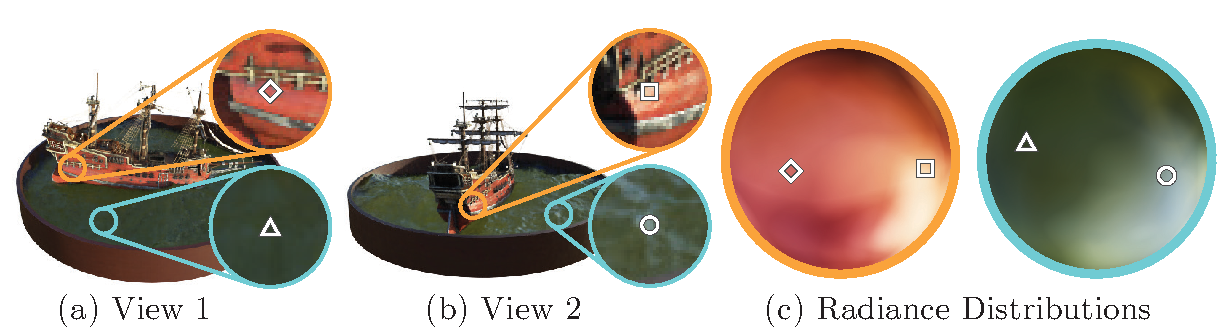
\includegraphics[width=\textwidth]{assets/viewdirs_small.pdf}
	\caption{С разных ракурсов в одном и том же месте кадра меняется цвет, попадаемый на пиксель}
	\label{fig:viewdirs_nerf}
\end{figure}

На рисунке \ref{fig:viewdirs_nerf} наглядно показано, что цвет одной и той же частички сцены может сильно варироваться от разного положения наблюдателя. Введение зависимости цвета от направления помогает решать эту проблему.

Выучивание специфики сцены ложится на MLP (многослойный перцептрон). По координатам $\mathbf x$ и направлению $\mathbf d$ он должен научиться выдавать такие параметры плотности $\sigma$ и цвета $C$, чтобы его рендер походил на целевые изображения.

Очевидно, что для рендера нужно в том числе знать и про положения камер, которые в оригинальной статье предлагается извлекать с помощью утилиты COLMAP \cite{schoenberger2016sfm}.

Также предлагается одновременно учить сразу 2 MLP:
%
\begin{itemize}
	\item первая сэмплирует точки равномерно на всей протяженности луча $[t_n, t_f]$, по которым определяется грубый цвет $C_c$ и вес каждой точки $w_i = T_i \left( 1 - e^{\sigma_i \cdot (t_{i+1} - t_i)} \right)$\footnote{Если точнее, то отрезок разбивается на N равных частей, и в каждой из этих частей равномерно выбирается по одной точке. Это позволяет всегда покрывать весь отрезок.};
	\item вторая сэмплирует точки согласно распределению, учитывающему веса $w_i$, полученные первой сетью, и дополняет цвет $C_c$ до итогового цвета $C_f$.
\end{itemize}
%
Первая сеть позволяет грубо оценить где реально имеет смысл считывать цвет и не тратить ресурсы в пустую. Это позволяет второй сети сэмплировать больше точек и при этом делать это максимально эффективно. Обе сети участвуют в обучении по метрике среднеквадратического отклонения
%
\[
	\mathcal{L} = \left( C_c - C_{g.t.} \right)^2 + \left( C_f - C_{g.t.} \right)^2,
\]
%
где $C_{g.t.}$ - это пиксель целевого изображения.

\begin{figure}
	\centering
	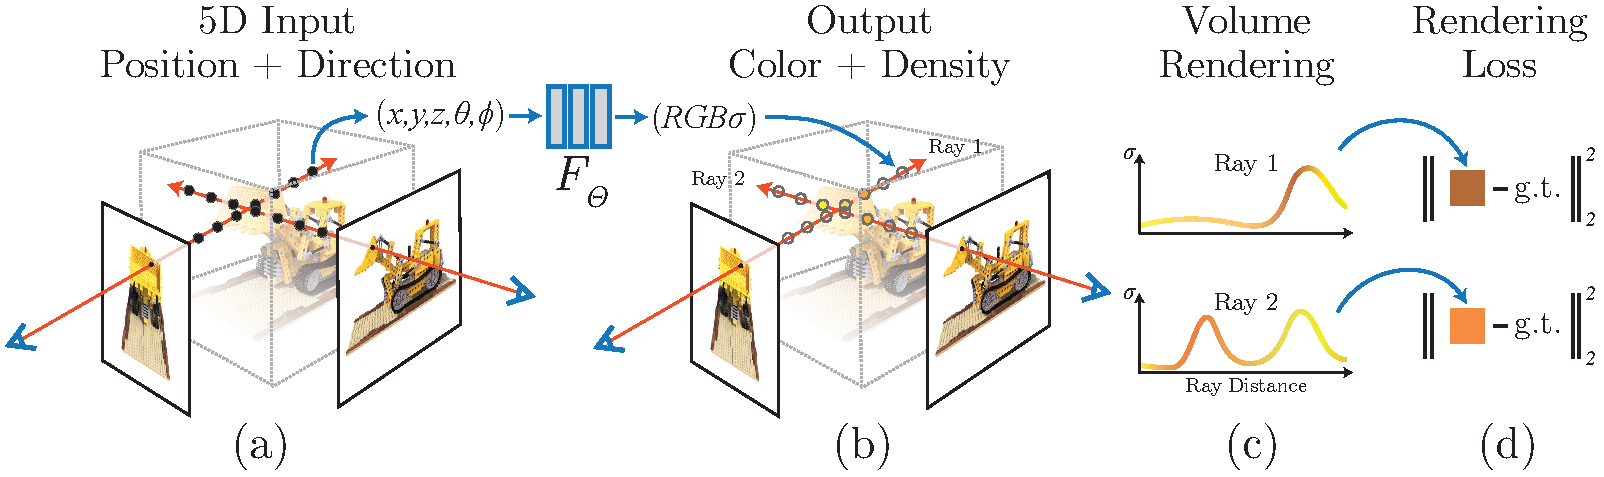
\includegraphics[width=\textwidth]{assets/pipeline_v2_small.pdf}
	\caption{Пайплайн обучения NeRF}
	\label{fig:nerf_pipeline}
\end{figure}

На рисунке \ref{fig:nerf_pipeline} приведено обучение NeRF.